\begin{figure}[!htb]
	\centering

	\begin{tikzpicture}

		\onslide<1->{
			\node (Before) at (0,0) {
				\begin{tikzpicture}[scale=0.15]
					\coordinate (1) at (-5,-8);
					\coordinate (2) at (10,2);
					\coordinate (3) at (10,10);
					\coordinate (4) at (-7,1);
					\coordinate (5) at (-1,8);
					\coordinate (6) at (-4,-9);
					\coordinate (7) at (5,-3);
					\coordinate (8) at (6,4);
					\coordinate (9) at (3,-5);
					\coordinate (10) at (0,1);

					\foreach \i in {1, ..., 10}{
							\filldraw[black] (\i) circle (4pt);
						}
				\end{tikzpicture}
			};
		}


		\onslide<2->{
			\node (NoDelaunay) at (4,1.5) {
				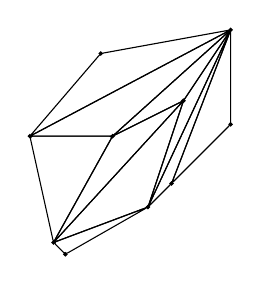
\begin{tikzpicture}[scale=0.15]
					\coordinate (1) at (-5,-8);
					\coordinate (2) at (10,2);
					\coordinate (3) at (10,10);
					\coordinate (4) at (-7,1);
					\coordinate (5) at (-1,8);
					\coordinate (6) at (-4,-9);
					\coordinate (7) at (5,-3);
					\coordinate (8) at (6,4);
					\coordinate (9) at (3,-5);
					\coordinate (10) at (0,1);

					\draw[rounded corners=1pt] (4) -- (3) -- (10) -- cycle;
					\draw[rounded corners=1pt](3) -- (8) -- (10) -- cycle;
					\draw[rounded corners=1pt] (3) -- (2) -- (7) -- cycle;
					\draw[rounded corners=1pt] (3) -- (7) -- (9) -- cycle;
					\draw[rounded corners=1pt] (3) -- (8) -- (9) -- cycle;
					\draw[rounded corners=1pt] (8) -- (9) -- (1) -- cycle;
					\draw[rounded corners=1pt] (1) -- (4) -- (10) -- cycle;
					\draw[rounded corners=1pt] (1) -- (8) -- (10) -- cycle;
					\draw[rounded corners=1pt] (1) -- (6) -- (9) -- cycle;
					\draw[rounded corners=1pt] (4) -- (3) -- (5) -- cycle;

					\foreach \i in {1, ..., 10}{
							\filldraw[black] (\i) circle (4pt);
						}
				\end{tikzpicture}
			};

			\node (NoDelaunayText) at (7,1.5) {\emph{Bad looking}};
			\draw[->, thick] (Before.east) -- (NoDelaunay.west);
		}
		\onslide<3->{
			\node (Delaunay) at (4,-1.5) {
				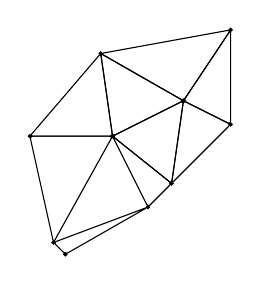
\begin{tikzpicture}[scale=0.15]
					\coordinate (1) at (-5,-8);
					\coordinate (2) at (10,2);
					\coordinate (3) at (10,10);
					\coordinate (4) at (-7,1);
					\coordinate (5) at (-1,8);
					\coordinate (6) at (-4,-9);
					\coordinate (7) at (5,-3);
					\coordinate (8) at (6,4);
					\coordinate (9) at (3,-5);
					\coordinate (10) at (0,1);

					\draw[rounded corners=1pt] (4) -- (5) -- (10) -- cycle;
					\draw[rounded corners=1pt] (1) -- (6) -- (9) -- cycle;
					\draw[rounded corners=1pt] (5) -- (8) -- (10) -- cycle;
					\draw[rounded corners=1pt] (7) -- (8) -- (10) -- cycle;
					\draw[rounded corners=1pt] (7) -- (9) -- (10) -- cycle;
					\draw[rounded corners=1pt] (2) -- (7) -- (8) -- cycle;
					\draw[rounded corners=1pt] (3) -- (5) -- (8) -- cycle;
					\draw[rounded corners=1pt] (2) -- (3) -- (8) -- cycle;
					\draw[rounded corners=1pt] (1) -- (4) -- (10) -- cycle;

					\foreach \i in {1, ..., 10}{
							\filldraw[black] (\i) circle (4pt);
						}
				\end{tikzpicture}
			};

			\node (DelaunayText) at (7,-1.5) {\emph{Nice looking}};

			% Arrow between them
			\draw[->, thick] (Before.east) -- (Delaunay.west);
		}

	\end{tikzpicture}

	\caption{A triangulation and a Delaunay triangulation in 2D}\label{fig:delaunayTriangulation}
\end{figure}
